\let\negmedspace\undefined
\let\negthickspace\undefined
\documentclass[journal]{IEEEtran}
\usepackage[a5paper, margin=10mm, onecolumn]{geometry}
%\usepackage{lmodern} % Ensure lmodern is loaded for pdflatex
\usepackage{tfrupee} % Include tfrupee package

\setlength{\headheight}{1cm} % Set the height of the header box
\setlength{\headsep}{0mm}     % Set the distance between the header box and the top of the text

\usepackage{gvv-book}
\usepackage{gvv}
\usepackage{cite}
\usepackage{amsmath,amssymb,amsfonts,amsthm}
\usepackage{algorithmic}
\usepackage{graphicx}
\usepackage{textcomp}
\usepackage{xcolor}
\usepackage{txfonts}
\usepackage{listings}
\usepackage{enumitem}
\usepackage{mathtools}
\usepackage{gensymb}
\usepackage{comment}
\usepackage[breaklinks=true]{hyperref}
\usepackage{tkz-euclide} 
\usepackage{listings}
% \usepackage{gvv}                                        
\def\inputGnumericTable{}                                 
\usepackage[latin1]{inputenc}                                
\usepackage{color}                                            
\usepackage{array}                                            
\usepackage{longtable}                                       
\usepackage{calc}                                             
\usepackage{multirow}                                         
\usepackage{hhline}                                           
\usepackage{ifthen}                                           
\usepackage{lscape}
\begin{document}

\bibliographystyle{IEEEtran}
\vspace{3cm}

\title{NCERT - 12.6.5.17}
\author{EE24BTECH11040 - Mandara Hosur}
% \maketitle
% \newpage
% \bigskip
{\let\newpage\relax\maketitle}

\renewcommand{\thefigure}{\theenumi}
\renewcommand{\thetable}{\theenumi}
\setlength{\intextsep}{10pt} % Space between text and floats


\numberwithin{equation}{enumi}
\numberwithin{figure}{enumi}
\renewcommand{\thetable}{\theenumi}

\textbf{Question:}\\
A square piece of tin of side 18 cm is to be made into a box without top, by cutting a square from each corner and folding up the flaps to form the box. What should be the side of the square to be cut off so that the volume of the box is the maximum possible? \\

\textbf{Solution (using gradient ascent):} \\
Gradient ascent is an optimization algorithm used to find the local maximum of a function. It iteratively moves in the direction of the steepest ascent, or the direction in which the function's value increases the most. \\
Let the side length of the square to be cut off be $x$ (where $0 < x < 9$, since $x$ cannot exceed half the side length of the square tin). After cutting the squares and folding the flaps, the dimensions of the box will be:
\begin{align}
\text{Length} = 18 - 2x, \quad \text{Width} = 18 - 2x, \quad \text{Height} = x.
\end{align}
The volume of the box, $V(x)$, is given by: 
\begin{align}
V(x) = x \cdot (18 - 2x)^2.
\end{align}
To maximize $V(x)$, compute its derivative $\frac{dV}{dx}$ and use gradient ascent to iteratively find the optimal value of $x$. \\
Expanding $(18 - 2x)^2$:
\begin{align}
(18 - 2x)^2 = 324 - 72x + 4x^2
\end{align}
Substituting this into $V(x)$:
\begin{align}
V(x) = x(324 - 72x + 4x^2) = 324x - 72x^2 + 4x^3
\end{align}
Differentiating $V(x)$ with respect to $x$:
\begin{align}
\frac{dV}{dx} = 324 - 144x + 12x^2
\end{align}
Using gradient ascent, we start with an initial guess $x_0$ (where $0 < x_0 < 9$) and a step size $\alpha > 0$. The update rule is:
\begin{align}
x_{n+1} = x_n + \alpha \frac{dV}{dx}\bigg|_{x = x_n} \\
\implies x_{n+1} = x_n + \alpha \brak{324 - 144x_n + 12x_n^2}
\end{align}
Ensure that $x$ remains within the bounds $0 < x < 9$ (as required for the given question). \\
The process stops when the change in $x$ between iterations is sufficiently small:
\begin{align}
|x_{n+1} - x_n| < \epsilon,
\end{align}
where $\epsilon$ is a small positive constant (e.g., $\epsilon = 10^{-6}$). \\
Since $x$ is bound, we can take $x_0 = 0$ and apply the method of gradient ascent.

\textbf{Solution (using manual methods):} \\
Using similar notations from above, we have:
\begin{align}
\frac{dV}{dx} = 324 - 144x + 12x^2 \label{derivative of volume expression}
\end{align}
For points of extrema, we need to equate \eqref{derivative of volume expression} to zero.
\begin{align}
324 - 144x + 12x^2 = 0 \\
\implies x = 9 \text{ and } x = 3
\end{align}
For the volume to be maximum, the derivative of the expression \eqref{derivative of volume expression} must be negative.
\begin{align}
\frac{d^2V}{dx^2} = 24x - 144 \label{double derivative of volume expression}
\end{align}
For $x=9$, equation \eqref{double derivative of volume expression} takes the value $72$, which is greater than zero. \\
For $x=3$, equation \eqref{double derivative of volume expression} takes the value $-72$, which is lesser than zero. This means that the maximum volume of the box is attained for this value of $x$. \\
Therefore, the length of the side of the square to be cut off so the volume of the box is the maximum possible is $3$ cm.

\newpage

\textbf{Plot:} \\
\begin{figure}[h]
	\centering
	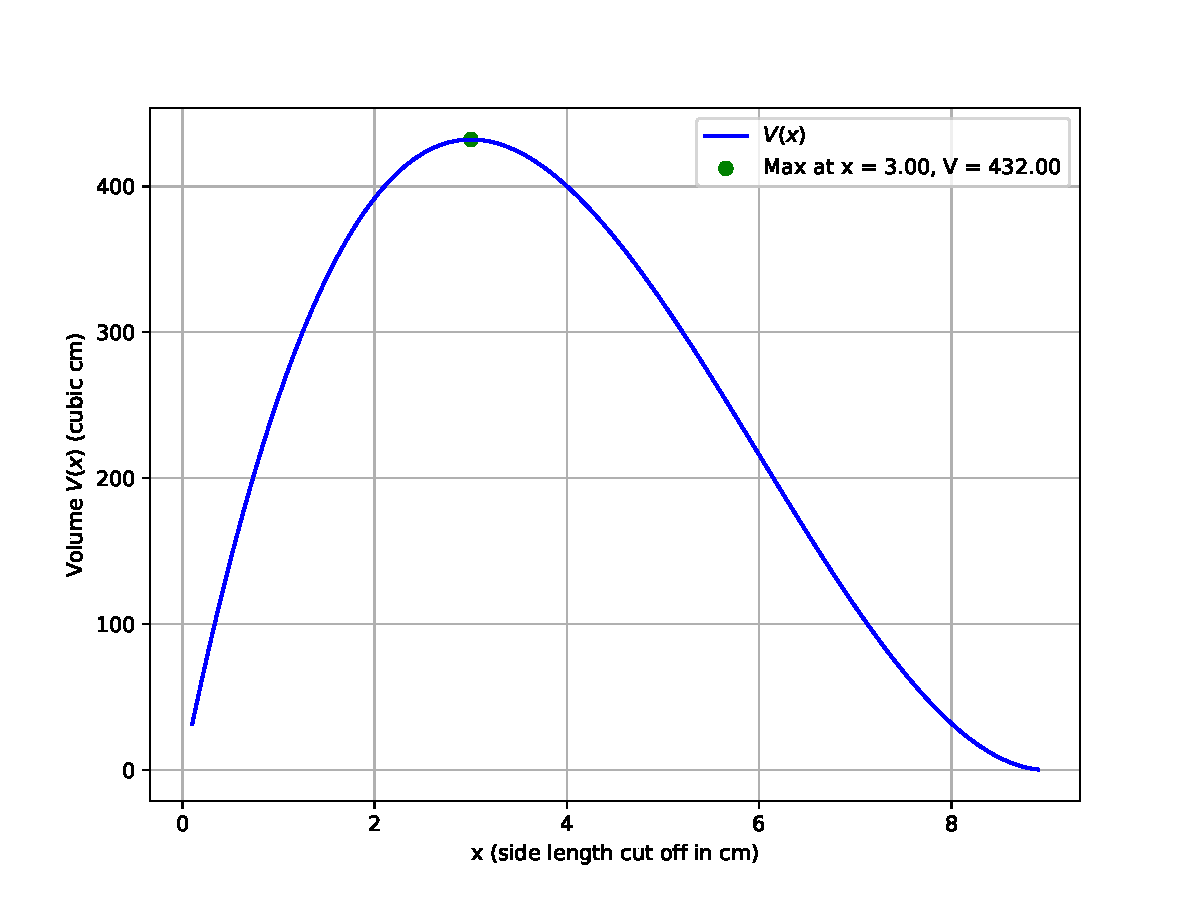
\includegraphics[width=\columnwidth]{figs/fig.pdf}
	\caption{Plot of Volume Function}
\end{figure}

\end{document}
